%%%%%%%%%%%%%%%%%%%%  練習問題（旧 prob_p8.png〜prob_p10.png）  %%%%%%%%%%%%%%%%%%%%
\newpage
\Rank{A問題}

\Mon{基本事項の確認}

\hspace{1zw}下図において，球体は静止している．また，(3)において，球体と斜面との間の摩擦は無視してよい．このとき，球体に作用している力を作図し，各々の力を「○○が△△に及ぼす××力」という形で答えよ（各々の力の大きさは求めなくてよい）．
\begin{center}
\begin{minipage}[t]{0.27\linewidth}
(1)\par\centering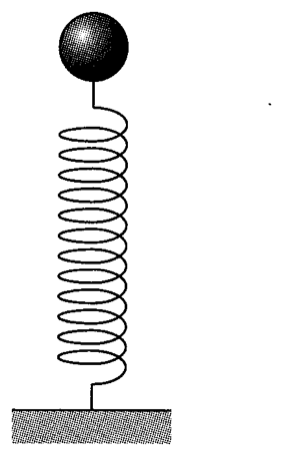
\includegraphics[keepaspectratio,width=20mm]{fig/ch3_p8_19a.png}
\end{minipage}\hfill
\begin{minipage}[t]{0.22\linewidth}
(2)\par\centering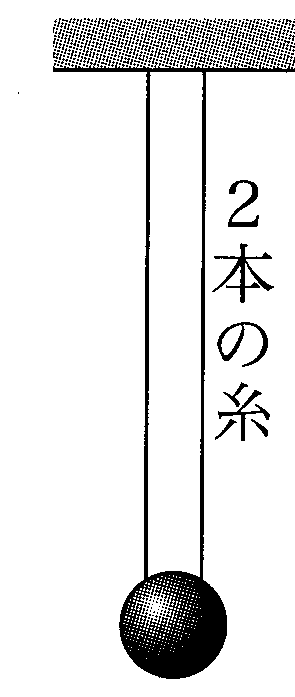
\includegraphics[keepaspectratio,width=14mm]{fig/ch3_p8_19b.png}
\end{minipage}\hfill
\begin{minipage}[t]{0.38\linewidth}
(3)\par\centering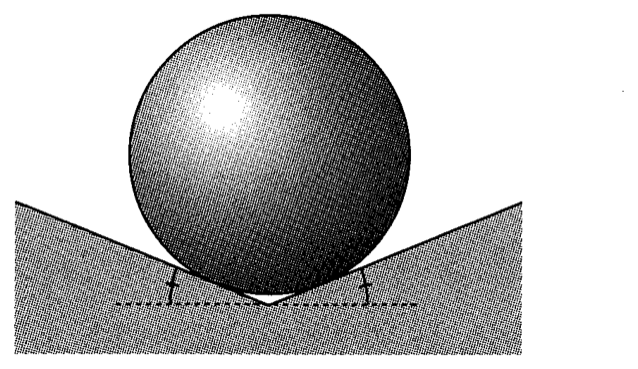
\includegraphics[keepaspectratio,width=45mm]{fig/ch3_p8_19c.png}
\end{minipage}
\end{center}

\Mon{基本事項の確認}

\begin{zuright}{43mm}
\hspace{1zw}机の上に板$\mathrm{B}$を置き，その上に物体$\mathrm{A}$を乗せる．次の力のうちで，
\begin{komon}
\ko{1} つり合いの関係にある力の組み合わせをすべて挙げよ．
\ko{2} 互いに作用・反作用の関係にある力の組み合わせをすべて挙げよ．
\end{komon}
\zusep
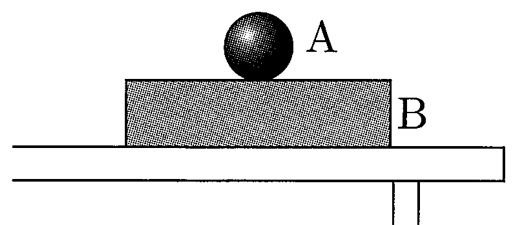
\includegraphics[keepaspectratio,width=36.5mm]{fig/ch3_p8_20.png}
\end{zuright}
\noindent\begin{tabular}{@{}p{0.49\linewidth}@{}p{0.49\linewidth}@{}}
\MARU{1}\quad 板$\mathrm{B}$が物体$\mathrm{A}$を押す力 &
\MARU{2}\quad 物体$\mathrm{A}$が板$\mathrm{B}$を押す力 \\
\MARU{3}\quad 板$\mathrm{B}$が机を押す力 &
\MARU{4}\quad 地球が物体$\mathrm{A}$を引く力 \\
\MARU{5}\quad 机が板$\mathrm{B}$を押す力 &
\MARU{6}\quad 地球が板$\mathrm{B}$を引く力 \\
\MARU{7}\quad 机が物体$\mathrm{A}$を押す力 &
\end{tabular}

\Rank{B問題}

\Mon{力のつり合い}

\begin{zuright}{62mm}
\hspace{1zw}右図のように，天井の2点$\mathrm{A}$，$\mathrm{B}$から糸$\mathrm{AC}$，$\mathrm{BC}$をぶら下げて質量$m\U{kg}$の物体をつり下げたところ，鉛直方向とそれぞれ$45^\circ$，$60^\circ$の角をなしてつり合った．このとき糸$\mathrm{AC}$，$\mathrm{BC}$の張力の大きさ$T_1$，$T_2$を求めよ．ただし，重力加速度の大きさを$g\U{m/s^2}$とする．
\zusep
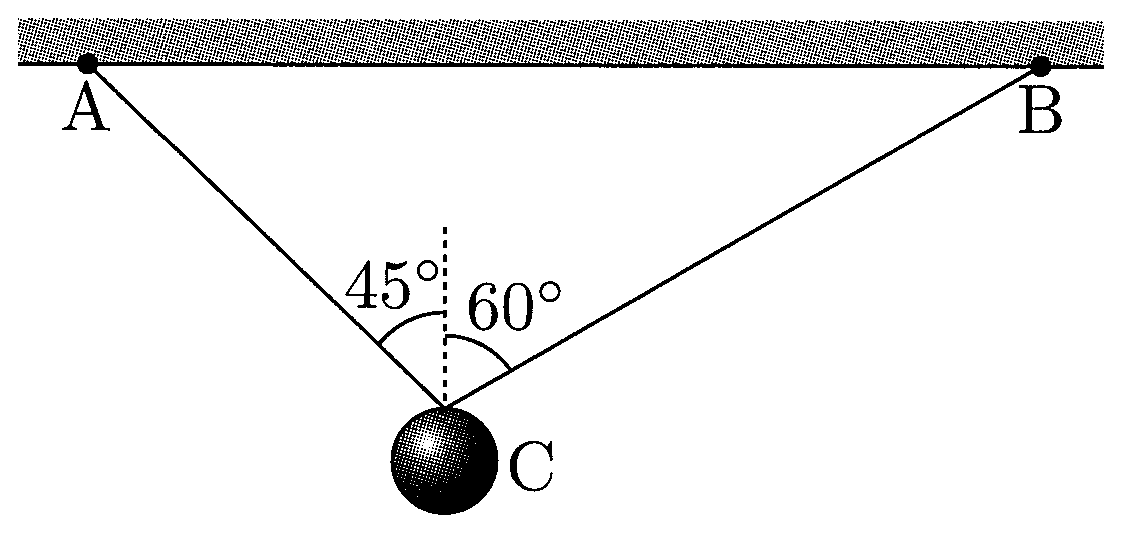
\includegraphics[keepaspectratio,width=51mm]{fig/ch3_p8_21.png}
\end{zuright}

\Mon{弾性力}\Sitei

\begin{zuright}{22mm}
\hspace{1zw}右図のように，質量が$m_1\U{kg}$のおもり$\mathrm{A}$と，質量が$m_2\U{kg}$のおもり$\mathrm{B}$を軽い糸と弾性定数$k\U{N/m}$の軽いばねでつるしたところ，ばねがある長さだけ伸びて各物体はつり合って静止した．重力加速度の大きさを$g\U{m/s^2}$として，以下の問いに答えよ．
\begin{komon}
\ko{1} 糸の張力の大きさを求めよ．
\ko{2} ばねの伸びを求めよ．
\end{komon}
\zusep
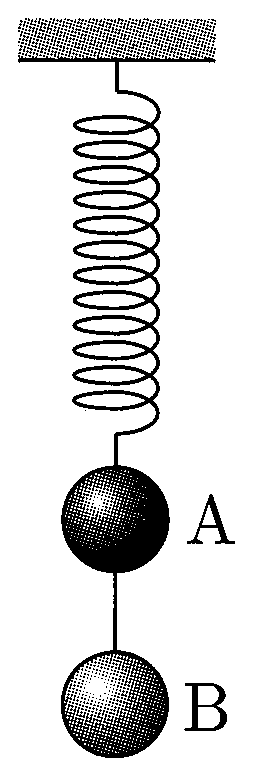
\includegraphics[keepaspectratio,width=12mm]{fig/ch3_p8_22.png}
\end{zuright}

\Mon{斜面上での最大摩擦力}

\begin{zuright}{52mm}
\hspace{1zw}右図のように，粗い面を持つ水平な板の上に質量$2.0\U{kg}$の物体を置き，水平方向に外力を加えたところ，外力が$8.0\U{N}$を越えると物体は板の上をすべり出した．重力加速度の大きさを$9.8\U{m/s^2}$として，以下の問いに有効数字2桁で答えよ．
\begin{komon}
\ko{1} 物体と板の間の静止摩擦係数を求めよ．
\ko{2} 板の上にこの物体を置いて，板を静かに傾けていく．物体がすべり始めるときの板の傾きを$\theta\U{rad}$とするとき，$\tan\theta$の値を求めよ．
\end{komon}
\zusep
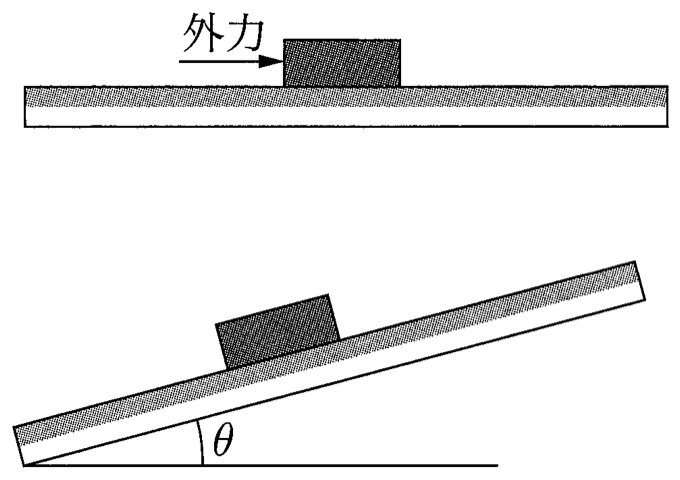
\includegraphics[keepaspectratio,width=48mm]{fig/ch3_p9_23.png}
\end{zuright}

\Mon{作用・反作用}

\begin{zuright}{35mm}
\hspace{1zw}次の文の空欄を適当な語句で埋めよ．

\hspace{1zw}台ばかりに物体$\mathrm{P}$をのせて質量を計ることができるのはなぜかを考えてみよう．重力加速度の大きさを$g\U{m/s^2}$，物体$\mathrm{P}$の質量を$m\U{kg}$とする．\MARU{3}\MARU{6}\MARU{7}は式で，その他は言葉で答えよ．

\hspace{1zw}物体$\mathrm{P}$には重力と\fbox{\MARU{1}}が作用しているが，物体$\mathrm{P}$が静止しているときにはこの二つの力は\fbox{\MARU{2}}の関係にあるので，\fbox{\MARU{1}}の大きさは\fbox{\MARU{3}}になる．

\hspace{1zw}さて，台ばかりの内部は図のように鉛直に取り付けられたバネの上に皿が乗っている構造になっており，前面の針はバネの縮みに応じて回転する仕組みになっている．台ばかりの皿は軽く，その質量を無視してよいものとして，皿に作用する力を考えると，皿にはバネからの弾性力と，\fbox{\MARU{1}}の\fbox{\MARU{4}}の関係にある力である\fbox{\MARU{5}}が作用する．そのため，この力によってバネは押し縮められる．弾性定数を$k\U{N/m}$，バネの縮みを$x\U{m}$とすると，皿に作用する力のつり合いの式は\fbox{\MARU{6}}となり，これからバネの縮みは\fbox{\MARU{7}}となる．よって，台ばかりの内部のバネの縮みの距離から，皿の上に乗っている物体の質量$m\U{kg}$を逆算することができる．
\zusep
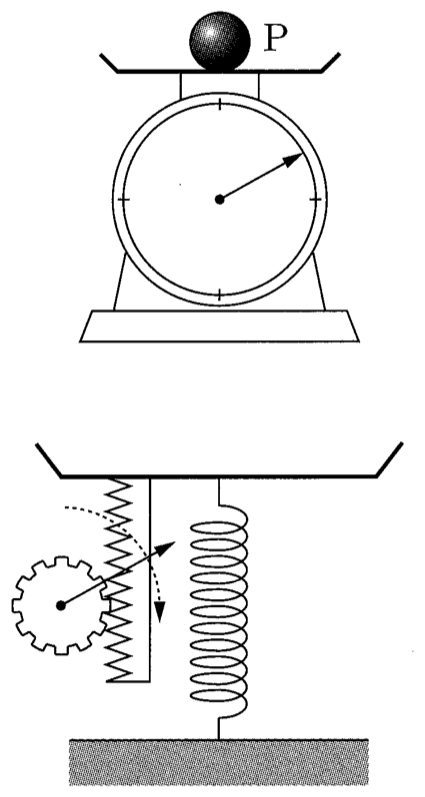
\includegraphics[keepaspectratio,width=30mm]{fig/ch3_p9_24.png}
\end{zuright}

\Mon{力のつり合い}\Sitei

\begin{zuright}{47mm}
\hspace{1zw}右図のように，仰角$30^\circ$のなめらかな斜面上に，天井から糸でつるした質量$m\U{kg}$の物体を置いたところ，糸が鉛直方向と$30^\circ$の角をなしてつり合った．糸の張力と，斜面から物体に作用する垂直抗力の大きさを求めよ．ただし，重力加速度の大きさを$g\U{m/s^2}$とする．
\zusep
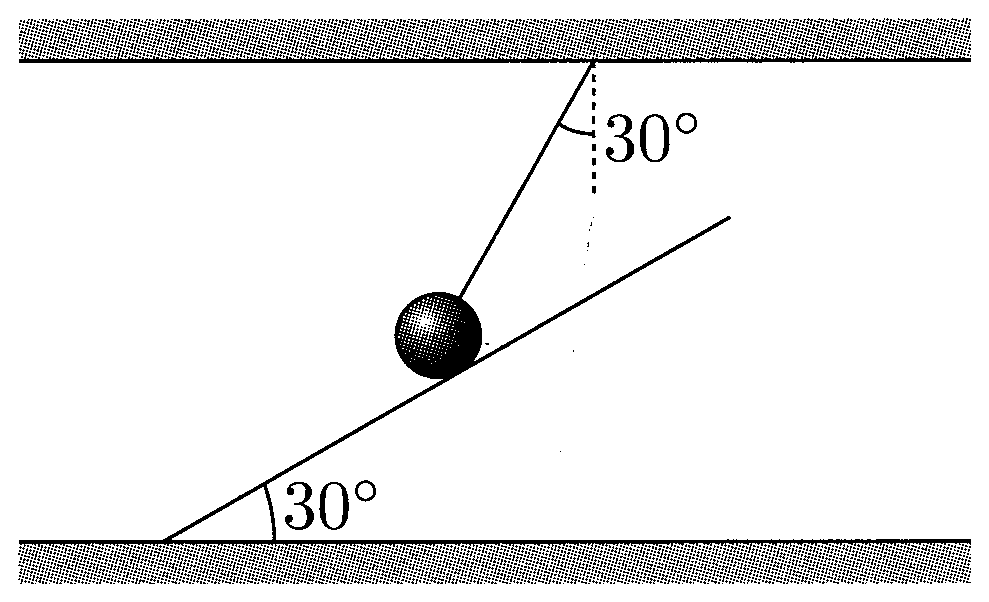
\includegraphics[keepaspectratio,width=47mm]{fig/ch3_p9_25.png}
\end{zuright}

\filbreak
\Rank{C問題}

\begingroup
\let\filbreak\relax
\Mon{弾性力}
\endgroup

\begin{zuright}{47mm}
\hspace{1zw}右図のように，自然長が$l\U{m}$でばね定数の等しいばね2本を，距離$2l\U{m}$だけ離して天井にとりつけ，2つのばねの下端をつないだ．2つのばねの先に，質量$m\U{kg}$のおもり$\mathrm{A}$をつないだところ，ばねは鉛直線と$45^\circ$の角をなしてつり合った．次に，質量$M\U{kg}$のおもり$\mathrm{B}$をつないだところ，ばねは鉛直線と$30^\circ$の角をなしてつり合った．$\mathrm{A}$と$\mathrm{B}$のおもりの質量の比$\dfrac{m}{M}$を求めよ．
\zusep
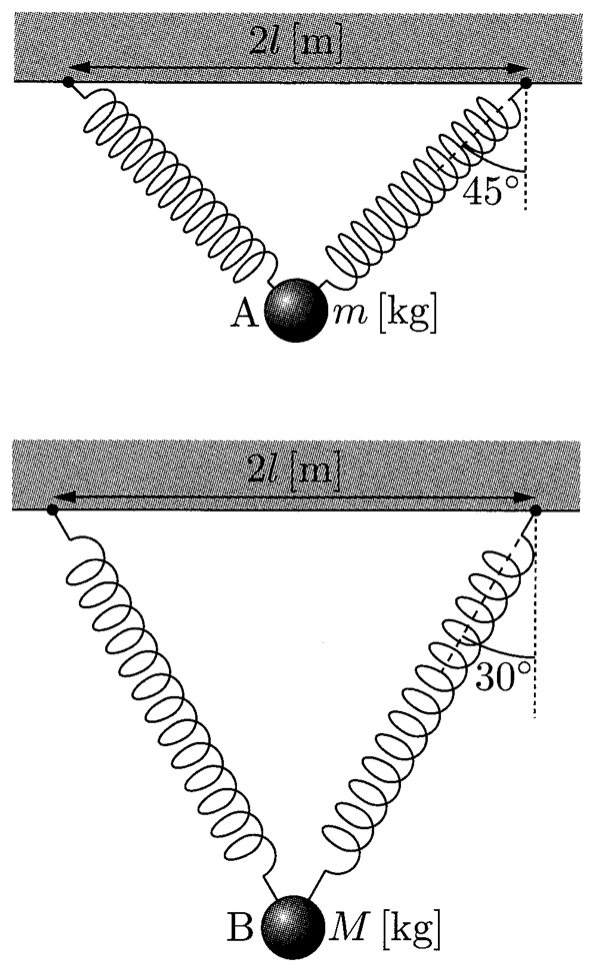
\includegraphics[keepaspectratio,width=42mm]{fig/ch3_p10_26.png}
\end{zuright}

\Mon{斜面上での最大摩擦力}

\begin{zuright}{47mm}
\hspace{1zw}右図のように，摩擦のある平板上に質量$m\U{kg}$の小物体が置かれている．重力加速度の大きさを$g\U{m/s^2}$として以下の問いに答えよ．
\begin{komon}
\ko{1} 板を静かに傾けていくと，板が水平面と角$\alpha_0$をなしたときに物体は滑り始めた．このことから，板と物体の間の静止摩擦係数$\mu_0$を$\alpha_0$で表せ．
\ko{2} 傾斜角を増して$\alpha\ (\alpha>\alpha_0)$にするとき物体が滑るのを防ぐためには，板面に平行上向きにどれだけの力を加えればよいか．その最小の力を求めよ．
\end{komon}
\zusep
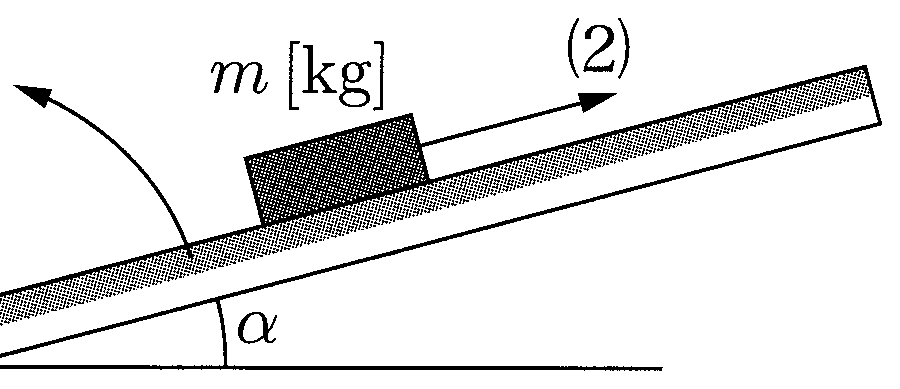
\includegraphics[keepaspectratio,width=42mm]{fig/ch3_p10_27.png}
\end{zuright}
